\section{課題2}

\subsection{パーセプトロン}

adaline.pyをオリジナルパーセプトロンに改良し，S層とA層の結合を追加した三層ネットワークを実装した．
S層→A層間の結合係数はランダムに$\{-1, 1\}$で固定し，活性化関数にはステップ関数を導入した．

\subsubsection{実行結果}

図\ref{fig:program7}に三層パーセプトロンの実行結果を示す．

\begin{figure}[htbp]
    \centering
    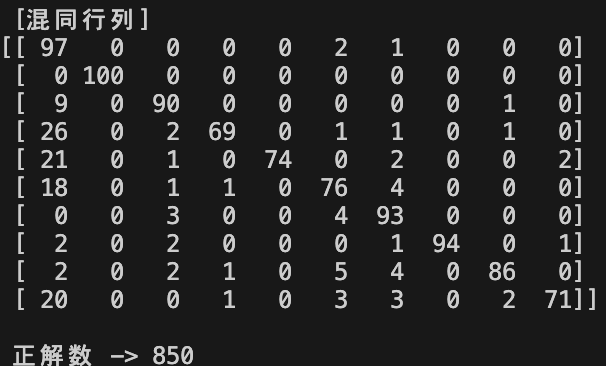
\includegraphics[width=0.8\linewidth]{fig/program-7_result.png}
    \caption{三層パーセプトロンの実行結果（混同行列と正解数）}
    \label{fig:program7}
\end{figure}

実行結果より，正解数は850/1000となり，正解率85.0\%を達成した．
元のADALINEの正解数750と比較すると，三層化により100サンプル分の精度向上が見られた．

\subsubsection{考察}

\paragraph{学習が収束しない理由}
ステップ関数は不連続であり微分不可能なため，勾配ベースの学習が理論的に成立しない．
これがADALINE（連続活性化関数を使用）との決定的な違いである．
実際の学習過程では，エポックごとの誤差が単調減少せず，振動や停滞が観察された．

\paragraph{S層→A層の固定結合の影響}
ランダムな$\{-1, 1\}$の結合係数により，入力空間からランダムな射影が行われる．
これは近年のReservoir ComputingやExtreme Learning Machineの考え方に通じるものであり，
ランダム射影によって入力の非線形な特徴抽出が可能となる．
隠れ層のユニット数を増やすことで，より多様な特徴を捉えられる可能性がある．

\paragraph{ADALINEとの比較}
ADALINEは連続な活性化関数を用いるため勾配降下法による学習が可能だが，
オリジナルパーセプトロンはステップ関数を用いるため，Hebbの学習則に基づく更新となる．
今回の結果では三層パーセプトロンがADALINEを上回ったが，
これはランダム射影による特徴空間の拡張効果と考えられる．


\subsection{誤差逆伝播法}

3層型ニューラルネットワークを用いて，CIFAR-10データセットの画像認識を行った．
訓練データ2,000枚で学習し，テストデータ2,000枚で評価を行った．

\subsubsection{実行結果}

図\ref{fig:program8}にテストデータに対する混同行列と認識結果を示す．

\begin{figure}[htbp]
    \centering
    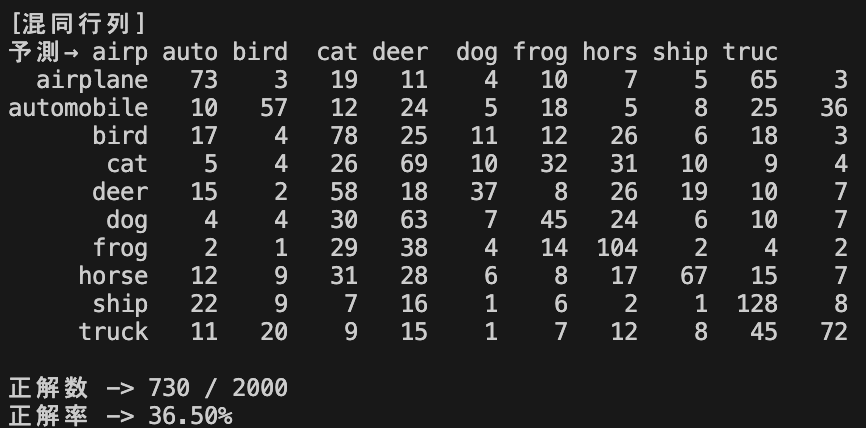
\includegraphics[width=0.9\linewidth]{fig/program-8_result.png}
    \caption{誤差逆伝播法による CIFAR-10 認識結果}
    \label{fig:program8}
\end{figure}

100エポックの学習後，テストデータに対する正解率は36.50\%（730/2000）となった．
学習過程では，損失が118.76から59.99まで減少し，訓練精度は68.70\%に達した．

\subsubsection{考察}

\paragraph{訓練精度とテスト精度の乖離}
訓練精度68.70\%に対してテスト精度36.50\%と大きな差があり，過学習が発生していると考えられる．
これは訓練データ数が2,000枚と比較的少ないことに起因する．
データ拡張やドロップアウトなどの正則化手法を導入することで，汎化性能の向上が期待できる．

\paragraph{クラス間の混同傾向}
混同行列を見ると，以下のような傾向が観察される：
\begin{itemize}
    \item shipは比較的高い精度（128/200）で認識されている．これは背景（海や空）の特徴が明確なためと考えられる．
    \item catとdogの混同が多い．両者は形状や色が類似しているため，3層ネットワークでは区別が困難である．
    \item deerは多くがbirdやfrogに誤分類されており，動物カテゴリ間での混同が顕著である．
\end{itemize}

\paragraph{ネットワーク構造の限界}
CIFAR-10は32×32のカラー画像であり，入力次元は3,072次元となる．
3層の全結合ネットワークでは空間的な特徴を効率的に抽出することが難しく，
畳み込みニューラルネットワーク（CNN）を用いることでより高い精度が期待できる．


\subsection{オートエンコーダ（主成分分析）}

Hebb学習（Sangerの学習則）を用いて，MNISTデータセットに対する主成分分析を行った．
10個の主成分を抽出し，画像の圧縮と復元を行った．

\subsubsection{実行結果}

図\ref{fig:program9}に学習過程の出力を，図\ref{fig:reconstruction}に元画像と復元画像の比較を示す．

\begin{figure}[htbp]
    \centering
    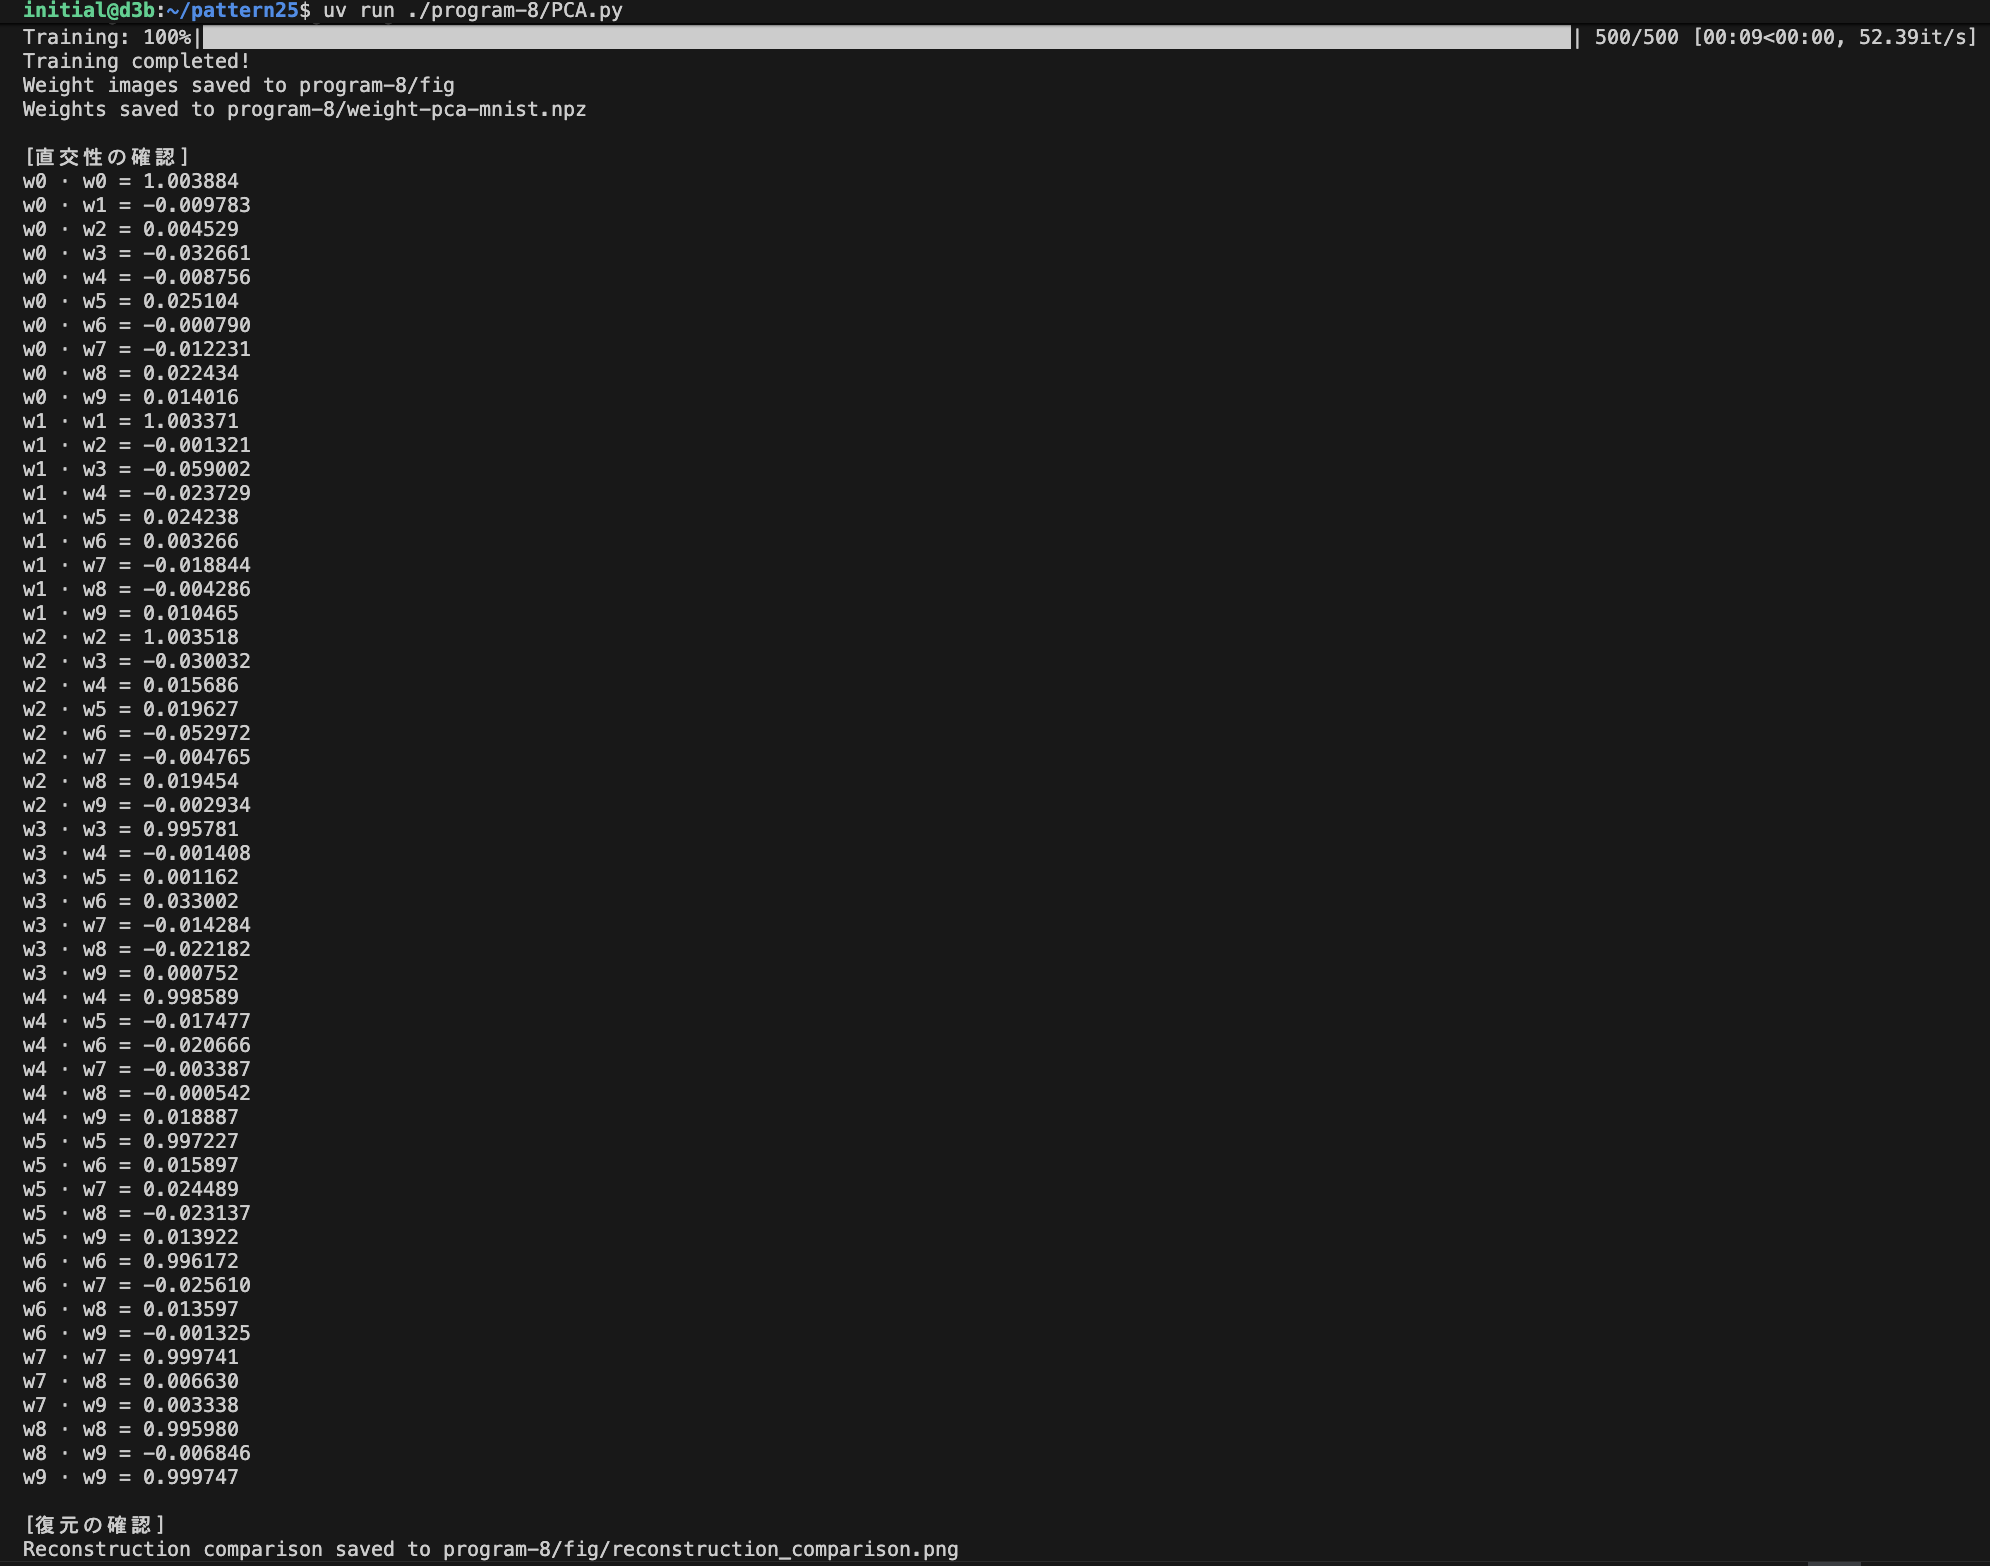
\includegraphics[width=0.8\linewidth]{fig/program-9_result.png}
    \caption{Hebb学習（Sangerの学習則）の実行結果}
    \label{fig:program9}
\end{figure}

\begin{figure}[htbp]
    \centering
    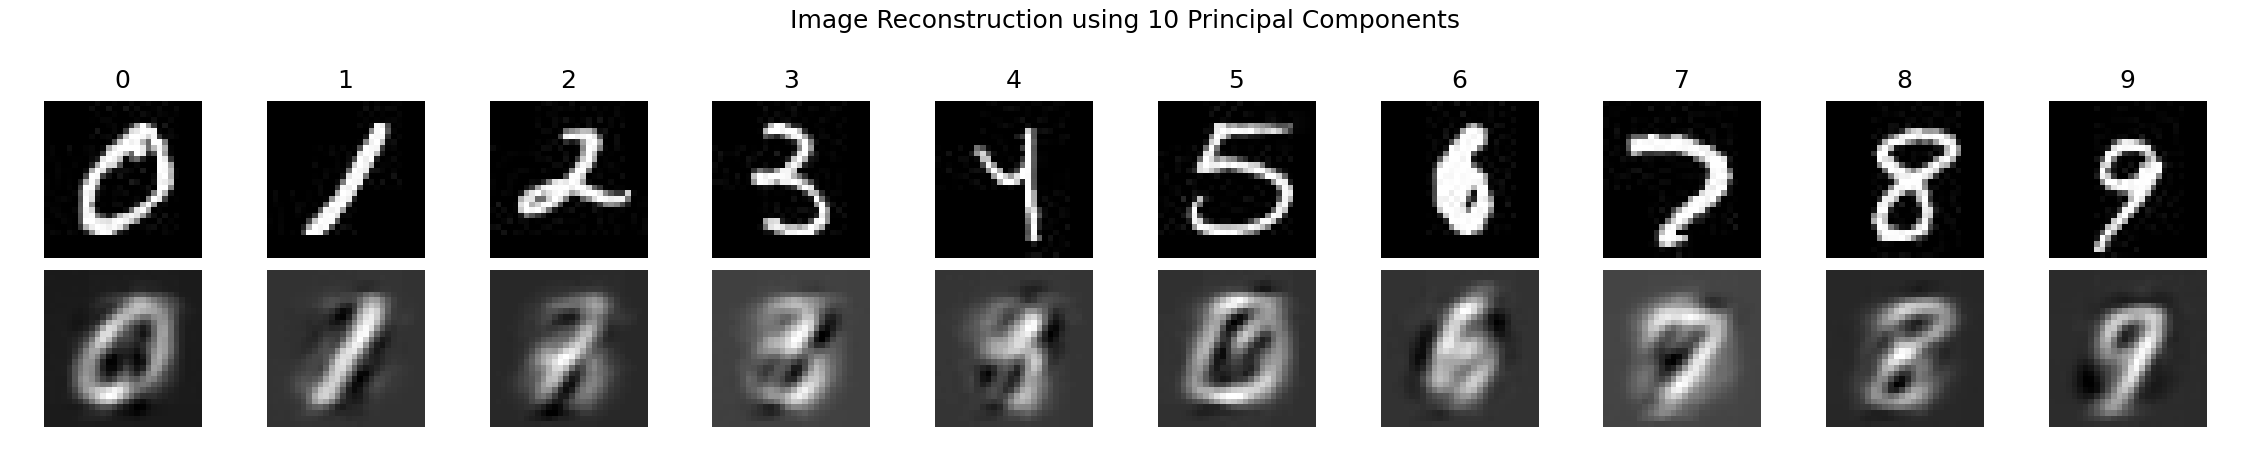
\includegraphics[width=\linewidth]{fig/program-9_result/reconstruction_comparison.png}
    \caption{10個の主成分による画像復元結果（上段：元画像，下段：復元画像）}
    \label{fig:reconstruction}
\end{figure}

\subsubsection{考察}

\paragraph{重みベクトルの直交性}
学習後の重みベクトル間の内積を確認すると，自己内積は約1.0（$w_i \cdot w_i \approx 1.0$），
異なるベクトル間の内積は約0（$w_i \cdot w_j \approx 0, i \neq j$）となっており，
Sangerの学習則により正規直交基底が獲得されていることが確認できた．
これは主成分分析の固有ベクトルに相当する．

\paragraph{復元品質の分析}
図\ref{fig:reconstruction}より，10個の主成分による復元結果を確認すると：
\begin{itemize}
    \item 0, 1は比較的良好に復元されている．これらは形状が単純で，少数の主成分で表現可能なためである．
    \item 4と9，2と3は両者の特徴が混合しているように見える．これらの数字は形状が類似しており，共通の主成分で表現される部分が多いためと考えられる．
    \item 5は円の要素が混入し，0のような見た目になっている．これは主成分が複数の数字クラスにまたがる特徴を捉えているためである．
\end{itemize}

\paragraph{次元圧縮率と復元誤差のトレードオフ}
元の画像は784次元（28×28）であり，10次元に圧縮することで約98.7\%の次元削減を実現している．
平均二乗誤差（MSE）は2147.85であり，完全な復元ではないものの，
数字の大まかな形状は保持されている．
主成分数を増やすことで復元品質は向上するが，圧縮率とのトレードオフとなる．
